\section{Problem 3}
\label{part3}
\begin{verbatim}
Estimate the age of each of the 1000 URIs using the ``Carbon Date'' tool:

http://ws-dl.blogspot.com/2014/11/2014-11-14-carbon-dating-web-version-20.html

Note: you'll should download the library and run it locally; don't
try to use the web service.

For URIs that have > 0 Mementos and an estimated creation date,
create a graph with age (in days) on one axis and number of mementos
on the other.  

Not all URIs will have Mementos, and not all URIs will have an estimated
creation date.  State how many fall into either categories

\end{verbatim}
\subsection{Solution}
\begin{enumerate}

\item Aim of this question is to find out the age of each url in days. But only those urls should be considered which have more than 0 mementos.
\item I already filtered all those urls with more than 0 mementos from my previous code and that file is given as input to the code written for this question. 
\item I referred the link given in the question and downloaded the carbon date tool zip file. From the link i got to know that there are 3 methods to find the created date of each link.
\item First one was web service which would take a whole lot of time to process my 177 urls. Other two were local.py and server.py.
\item I randomly picked local.py and understood the code. There was already one function defined which takes url as argument and give creation date and many other parameters as output.
\item Now I opened my file with 177 urls and ran a loop which took each url and called the above function and each time i appended my created date for each url to my output file.
\item Figure 7 shows my output json file which has url and its respective creation date. 
\item Now my task was to write code for calculation age of the url and this can be done by subtraction the creation date of the url from the present date.
\item Here i got stuck up for a lot of time while subtracting date there was constantly one error called some kind of valueError. 
\item I searched for this error in Google and got to know that i should use strptime function in order to modify my creation date format into present date's format. This command eliminated `T' variable which was present in our creation date.
\item Now i was successful in finding the age of each url in days and saved that to a csv file which shown below in Figure 8. I had also got number of mementos into a separate csv file so that i can easily pass my inputs to R.
\item Number of mementos saved in csv file is shown in Figure 9.
\item From the second question i already got some grip on R, so now i was able to pass the age and number of mementos as inputs to R which gave me a scatter plot as output.
\item Now this scatter plot shows that higher the number of mementos for a particular url higher is the age of that url. I had a maximum of 8999 mementos for 1 url and maximum age for 1 url was 6922 days.
\item The scatter plot is shown below in Figure 10.
\end{enumerate}
\newpage
\subsection{Code Listing}

\subsubsection{Python code for calculating creation date for each url}
\lstinputlisting[language=Python,breaklines = true,frame=single,caption={Python program for getting creation date for URI's}, label=lst:q1-1,captionpos=b,numbers=left,showspaces=false,showstringspaces=false,basicstyle=\footnotesize]{local.py}
\subsubsection{Python Code for Calculation age}
\lstinputlisting[language=Python,breaklines = true,frame=single,caption={Python program for calculating the age of URI's}, label=lst:q1-1,captionpos=b,numbers=left,showspaces=false,showstringspaces=false,basicstyle=\footnotesize]{cal_age_days.py}
\newpage
\subsubsection{R code for scatter plot}
\lstinputlisting[language=R,breaklines = true,frame=single,caption={R program for generating the scatter plot for Question 3}, label=lst:q2R,captionpos=b,numbers=left,showspaces=false,showstringspaces=false,basicstyle=\footnotesize]{scatter.R}
\subsection{Results}

\subsubsection{Creation date of each URL}
\begin{figure}[ht]    
    \begin{center}
        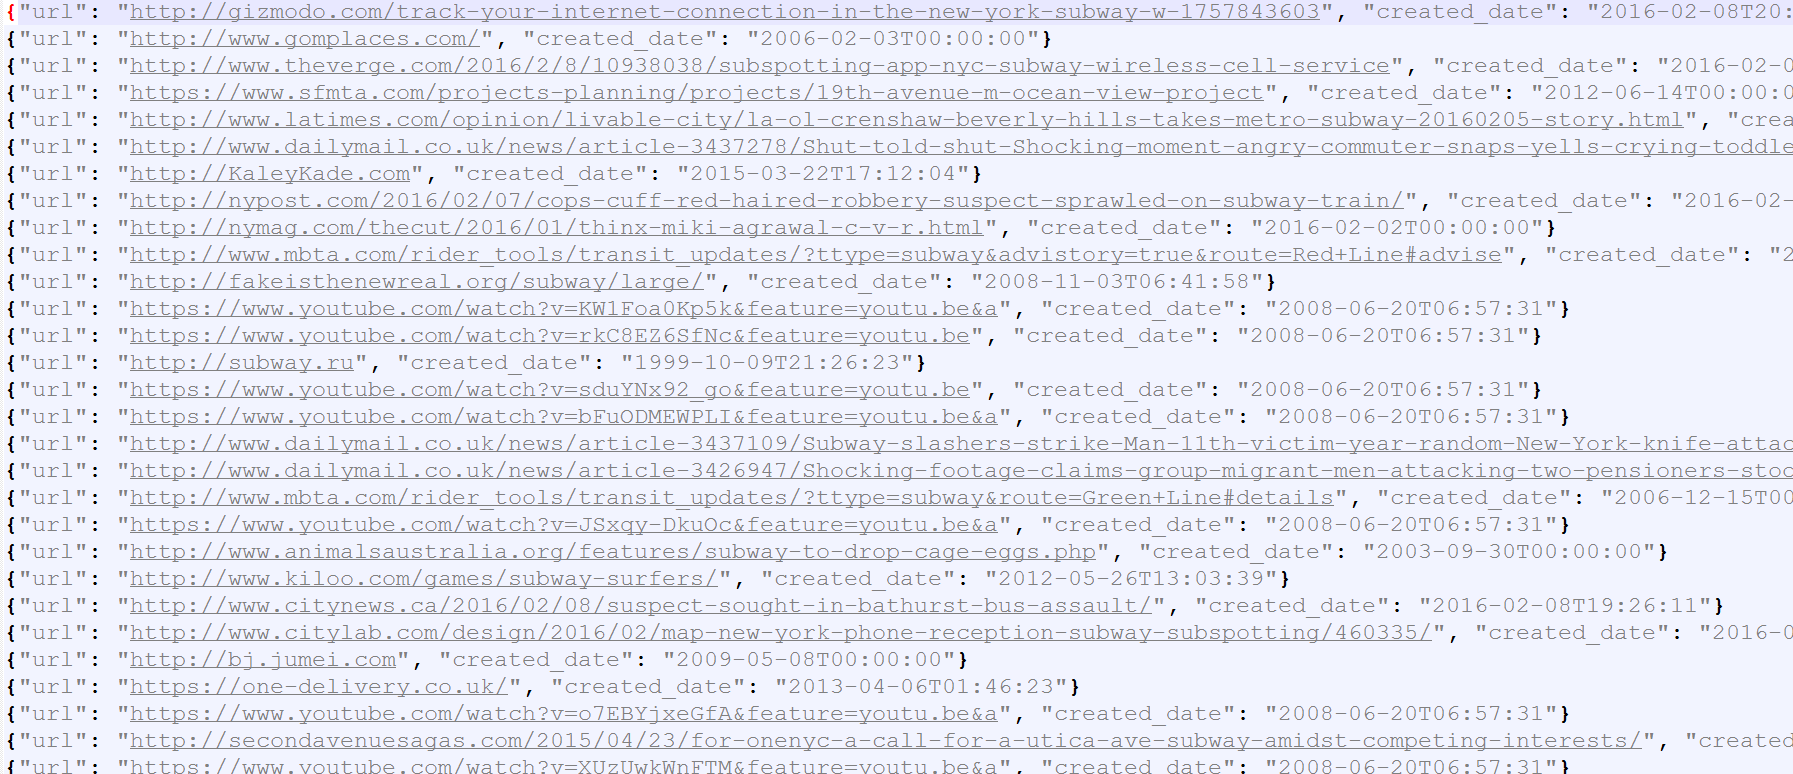
\includegraphics[scale=0.37]{url_creationdate.png}
        \caption{Each Url along with its creation date}
        \label{Each Url along with its creation date}
    \end{center}
\end{figure}
\newpage

\subsubsection{Age of each url}
\begin{figure}[ht]    
    \begin{center}
        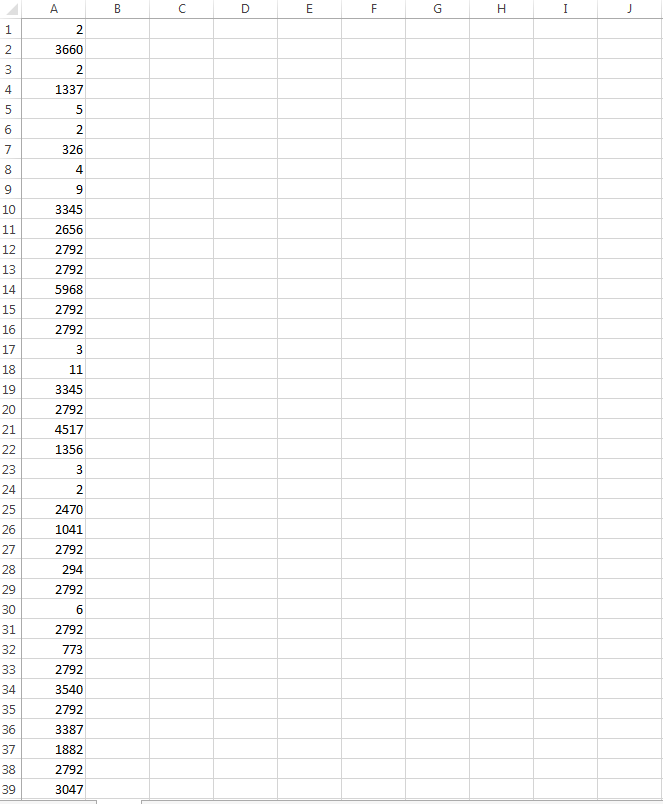
\includegraphics[scale=0.80]{age_in_days.png}
        \caption{Age of each url}
        \label{Age of each url}
    \end{center}
\end{figure}
\newpage

\subsubsection{Number of Mementos for each url}
\begin{figure}[ht]    
    \begin{center}
        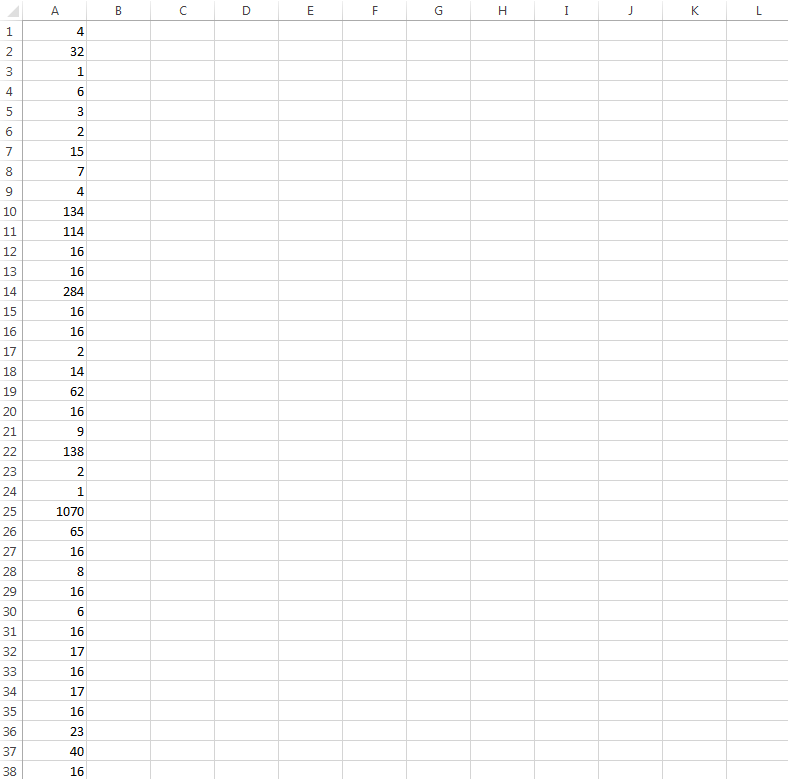
\includegraphics[scale=0.80]{num_mem.png}
        \caption{Number of Mementos for each url}
        \label{Number of Mementos for each url}
    \end{center}
\end{figure}
\newpage

\subsubsection{Q3-scatterplot}
\begin{figure}[ht]    
    \begin{center}
        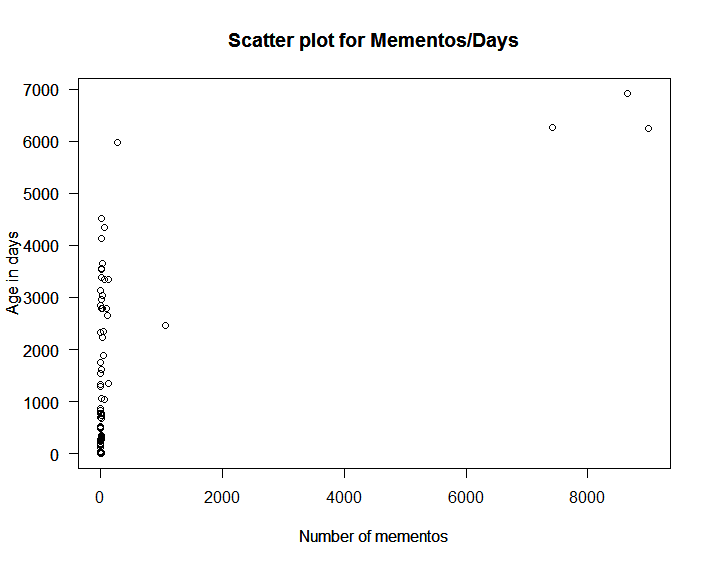
\includegraphics[scale=0.60]{scatter_age_mementos.png}
        \caption{ScatterPlot}
        \label{scatterPlot}
    \end{center}
\end{figure}